% GMW: Alice shares her input; the circuit invariant (2134 x 784 px); the circuit is a crop
\figsetup{2134}{784}%
\begin{tikzpicture}[fig]
\figbbox
\node[at base] at (8,230) {\fs{34}\fit{365}{Choose random \sbf{x\textsubscript{2}}}};
\node[at base] at (84,343) {\fs{34}\fit{197}{\sbf{x\textsubscript{1}=x\textsubscript{2}+x}}};
\icon{29}{428}{212}{720}{\pcalice}
\icon{757}{420}{965}{724}{\pcbob}
\draw[green!40!black, arr={3}{24}{22}] (406,506) -- (699,506);
\node[at base] at (528,452) {\fs{34}\sbf{x\textsubscript{2}}};
\node[anchor=north west] at (1338,93) {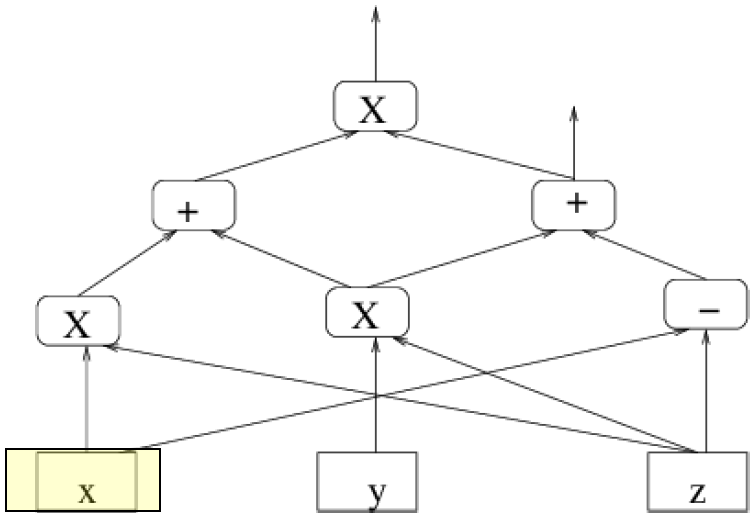
\includegraphics[width=755\fu]{figures/chapter-7-gmw-circuit-invariant-circuit.png}};
\node[at base] at (1671,62) {\fs{38}\fit{76}{Bob}};
\node[at base] at (1362,666) {\fs{38}\fit{95}{Alice}};
\node[at base] at (1671,666) {\fs{38}\fit{95}{Alice}};
\node[at base] at (1994,666) {\fs{38}\fit{78}{Bob}};
\end{tikzpicture}%
